\documentclass[lettersize,journal]{IEEEtran}
\usepackage{amsmath,amsfonts}
\usepackage{algorithmic}
\usepackage{algorithm}
\usepackage{array}
\usepackage[caption=false,font=normalsize,labelfont=sf,textfont=sf]{subfig}
\usepackage{textcomp}
\usepackage{stfloats}
\usepackage{url}
\usepackage{verbatim}
\usepackage{graphicx}
\usepackage{cite}
\hyphenation{op-tical net-works semi-conduc-tor IEEE-Xplore}
\usepackage{booktabs}
\usepackage{amsmath,amsfonts}
\usepackage{algorithmic}
\usepackage{array}
\usepackage{textcomp}
\usepackage{stfloats}
\usepackage{subcaption}
\usepackage{url}
\usepackage{verbatim}
\usepackage{graphicx}
\usepackage{float}
\usepackage{titlesec}
\usepackage{amsthm}
\usepackage{mathtools}
\usepackage{gensymb}
\usepackage{hyperref}
\usepackage{amssymb}
\usepackage{amsmath}
\usepackage{dsfont}


\newcommand{\rEarth}{R_{\oplus}}
\newcommand{\viiva}{\mathop{\Bigg/}}
\newcommand{\sij}[3]{\viiva\limits_{\hspace*{-5mm}{#1}}^{\hspace*{5mm}{#2}}{#3}}
\newcommand{\R}{\mathbb{R}}
\newcommand{\N}{\mathbb{N}}
\newcommand{\B}[1]{\mathbf{#1}}
\newtheorem{theorem}{Theorem}
\newtheorem{corollary}{Corollary}
\newtheorem{lemma}[theorem]{Lemma}
\newtheorem{prop}[theorem]{Proposition}
\newtheorem*{remark}{Remark}

\def\BibTeX{{\rm B\kern-.05em{\sc i\kern-.025em b}\kern-.08em
    T\kern-.1667em\lower.7ex\hbox{E}\kern-.125emX}}
\begin{document}

\title{Factorial moment measure of the SIR and Successive Interference Cancellation in a Narrow-Beam LEO Uplink}
\author{IEEE Publication Technology,~\IEEEmembership{Staff,~IEEE,}
        % <-this % stops a space
\thanks{This paper was produced by the IEEE Publication Technology Group. They are in Piscataway, NJ.}% <-this % stops a space
\thanks{Manuscript received October 8, 2023; revised December 8, 2023.}}

% The paper headers
\markboth{Journal of \LaTeX\ Class Files,~Vol.~1, No.~2, December~2023}%
{Shell \MakeLowercase{\textit{et al.}}: A Sample Article Using IEEEtran.cls for IEEE Journals}

\IEEEpubid{}
% Remember, if you use this you must call \IEEEpubidadjcol in the second
% column for its text to clear the IEEEpubid mark.


\maketitle
\begin{abstract}

  Based on a stationary Poisson point process (PPP) on the plane, a Gaussian (squared exponential) path loss, and a defective exponential fading distribution function, we approximate a narrow-beam Low Earth Orbit (LEO) uplink with a two-tier Gaussian mixture shadowing. We examine the process formed by the signal-to-interference ratios (SIRs) and signal-to-interference-plus-noise ratios (SINRs) of the ordered first $k$ user equipments with the strongest signals at the typical LEO base station (BS) by deriving the joint pdfs of the $k$th order statistics; characterized by the $k$th factorial moment measures. Strikingly, we are able to describe the total interference by a gamma process, resulting in a Poisson-Dirichlet distribution and a convenient mathematical expression for the pdf of the SIR order statistics. Furthermore, using the joint pdfs of the SIR and SINR order statistics, we examine the SIR and SINR under different signal cancellation scenarios. The analysis and mathematical expressions offer insights and a framework to conviently study the SIR and SINR of all transmitters and interference cancellation in LEO systems for different settings. We present multiple numerical results and validate the theoretical values with simulations based on a realistic system model utilizing PPP on the Earth surface and Gaussian mixture shadowing. Importantly, we demonstrate that interference cancellation can reduce the variance in the user experience of the link quality while maintaining the average performance over LEO BSs in a uniform constellation (\textit{i.e.}, improve user fairness).


\end{abstract}

% Note that keywords are not normally used for peerreview papers.
\begin{IEEEkeywords}
  
\end{IEEEkeywords}


\section{Introduction}
The steady rise of aerial communication networks, including LEO networks, owing to the planning and deployment of dense LEO networks to handle increased user-data as well as the expansion of the terrestrial frequency bands to those that are so far assigned only for the satellite communications, drives a need for new analytical tools to study and locate the essential properties of the networks. The signal-to-interference-plus-noise ratio SINR (or without the noise simply SIR) is a key metric, determinining the performance of the satellite link. A derivation of the SINR is, for example, spectral efficiency. The SINR is a function of propagation effects, which incorporates the distance-dependent path loss, fast-fading, slow-fading (shadowing), and a variety of atmospheric scattering and absorbion effects, etc. Altough not optimal, the analytic models, such as stochastic geometry models, often compromizes between analytical tractability and realism in the signal propagation model. Another cmmon simplification is to use the Poisson point process (PPP)---being the most tractable in the stochastic geometry analysis. Furthermore, as the points in the PPP are independently located, it can be a highly realistic model in scenarios such as in modeling the random locations of mobile user equipments (UEs), as the mobile phone user are more or less located independently from one another (as opposed to base stations (BSs), including LEO BSs, that are often more regularly located). However, the PPP works as a approximation also with many regular configurations. [CITE] The PPP has also a special role in the theory of point processes: any subsequentive independent random replacement of any point process (p.p.) will lead to the PPP. Furthermore, random multipath propagation effects can make a arbitrary p.p. to seem Poisson. [CITE]. However, often these simplifications don't detract from the statistical system-level insights the models introduce in simpler and more general terms compared to sophisticated scenario-specific simulations. The simple insights derived from the analytical models are important in comprehending the LEO networks and ultimately lead to more optimal allocation of simulation resources.


 However, in this work, we interpret the results in a narrow-beam LEO context. We validate the flat-Earth assumption and the simplified fading model, imposed in order to derive the mathematical results, by Monte Carlo simulating the realistic LEO network using spherical Earth model and Gaussian mixture shadowing.








\begin{table}
  \begin{center}
    \begin{tabular}{|c|p{4.5cm}|p{1.9cm}|}
      \multicolumn{3}{c}{\textbf{Principal symbols the values and units in the numerical results}} \\
      \toprule
      \multicolumn{3}{|c|}{\scriptsize{We denote (approximate) proportionality ``$\propto$'' or equality ``$=$'' to a variable.}} \\
      \multicolumn{3}{|c|}{\scriptsize{For a dimensional number, we denote the units ``SI'' and ``[non-SI].'' }} \\ 
      \hline
      Symbol& Explanation &Values and units
      \\ 
      \hline 
      $h$ & Receiving LEO BS altitudes. &$1200$ km  \\
%      $G[\cdot]$ &Gaussian antenna gain of a BS.&$\R_+ \rightarrow (0,1)$ \\
      $\alpha$ &Power path loss exponent.& $4$\\
      %% $\Phi\subset \R^2$ &Homogeneous PPP on planar Earth. & $\{(x_i,y_i)\}$ km\\
      %% $\Theta \subset \R^3 $ & Homogeneous PPP on spherical Earth surface of average radius $\rEarth=6378$. &$\{(\rEarth,\phi_i,\varphi_i)\}$\break (km, rad, rad) \\
      $\lambda$ & The density of $\Phi$ and $\Theta$, \textit{i.e.}, the mean number of UEs inside an unit area.&$\{4.6,8.8\}\break10^{-4}\text{/km}^2$\\
      $\epsilon$& The typical LEO BS elevation angle w.r.t $\textit{o}$.&$\left({\pi}/{2},{2\pi}/{9}\right)\text{ rad}\break=(90,40)[\degree]$\\
      %% $\kappa$  & Average number of  the LEO BS $-3 \text{ dB footprints};$& \\
      %% ${\tilde{\kappa}}$ &  $\kappa/\log(2)$.& \\
      $p_{\text{LoS}}$& LoS probability; $p_{\text{LoS}} \propto \sin(\epsilon)$. & $(0.99,0.61)$\\
%      $p_{\text{NLoS}}$& NLoS probability; $1-p_{\text{LoS}}$. & \\
      $\mu_{\text{LoS}}$& Mean of the LoS component of the Gaussian mixture shadow fading model. & $0$ [dB] \\
      $\mu_{\text{NLoS}}$& Mean of the NLoS component. & $-26$ [dB] \\
      $\sigma^2_{\text{LoS}}$& Variance of the LoS component. & $4^2$ [dB] \\
      $\sigma^2_{\text{NLoS}}$& Variance of the NLoS component. & $6^2$ [dB] \\
      %% $H_{\mathcal{M}\mathcal{L}\mathcal{N}}$ & A r.v. distributed according to a two-tier $\{\text{LoS}, \text{NLoS}\}$ log-normal mixture distribution representing the power fading.&   \\
      %% $H_{\text{Exp}}$ & A simple approximation of (mean normalized) $H_{\mathcal{M}\mathcal{L}\mathcal{N}}$. It has a defective exponential cdf entirely characterized by the atomic prob. measure at $0$; $1-\upsilon$.&\\
      %% $\upsilon$ & $\mathbb{P}(H_{\text{Exp}}>0)$ $=1-\mathbb{P}(H_{\text{Exp}}=0)$; $\upsilon = \upsilon(p_{\text{LoS}}(\epsilon))=v(\epsilon)$. &$(0.85,0.53)$ \\
      %% $\kappa \upsilon$ & The mean number of effective UEs inside the $-3$ dB footprints. \textbf{The parameter determines the theoretical SIR performance.}&$ \{1.8,2.6\}$ \\
      $\varphi_{\text{RX}}$ & Half-width of a LEO BS $-3$ dB antenna gain. $\varphi_{\text{RX}} = 0.028 \sin^{3/2}(\epsilon).$&$(.014,.028) \text{ rad}\hfill\break (0.8,1.6)[\degree]$ \\      
      $\kappa$& Average number of UEs inside a $-3$ dB footprint; $\kappa \propto \lambda, \kappa \propto 1/\sin(\epsilon)$.& 2.6 \\
      $\upsilon$&Fraction of effective UEs; $\hfill \break\upsilon \propto p_{\text{LoS}} \propto\sin(\epsilon),  \upsilon \propto \lambda$. & \\      
      $\kappa \upsilon$& Average number of effective UEs inside a $-3$ dB footprint; $\kappa \upsilon \propto \lambda $ .& $\{1.4,2.6 \}$ \\
      $\theta$ & SIR threshold of a successful transmission.&$(0.2,10)$  \break \hfill $(-7,10)$ [dB]   \\
      $\tau$ & SIR threshold of a successful interference cancellation.& $0.2$, $-7\text{ [dB]}$\\  
      \hline
    \end{tabular}
  \end{center}
\end{table}   


\section{System model}

\begin{figure}[h]%
  \centering
  \subfloat[\centering  Interpretation of the \textit{planar} system model with the satellites in adjacent orbits serving an urban area and a realization of the UEs. The altitudes are not to scale.]{{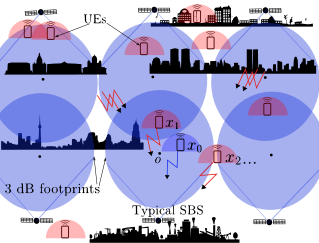
\includegraphics[width=\linewidth]{UEsontheplane.png}}
    \label{fig:UEsontheplane}%%
  } 
  \qquad
  \subfloat[\centering The typical LEO BS as seen from the side. The transmitters are projected into line $(0, \infty)$ according to their norm.]{{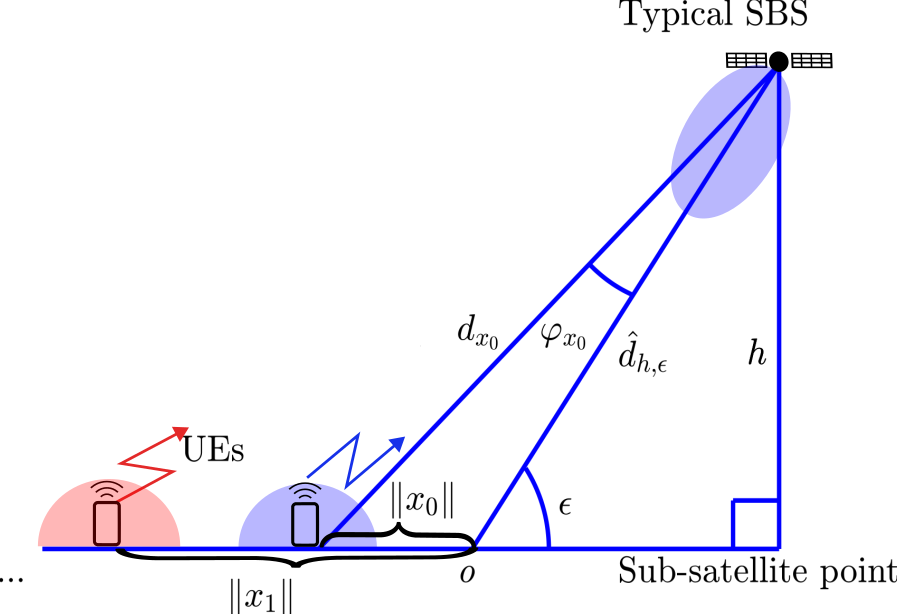
\includegraphics[width=\linewidth]{drawing.png}}     \label{fig:systemmodel}} %%
  \caption{The simplified narrow-beam LEO uplink system model. The satellite antenna boresight is oriented towards $\textit{o}$, the focus point of the elliptical footprint. The omnidirectionally transmitting UEs $\{x_i\}$ are located according to the HPPP on the plane. The nearest transmitter, $x_0$, is the served UE.}
\end{figure}




\label{sec:analysissec}




\subsection{Poisson process on the plane}
\label{sec:gainprocess}


Considering a uplink, the UEs follow a homogeneous PPP $\Phi \subset \R^2$ of density $\lambda$. The BSs form an independent homogeneous p.p. possibly with different density than the UEs. Because of the translation invariancy of the PPP, all location are statistically equivalent, and we define the origin $\textit{o}$ to represents the typical LEO BS footprint focus point.

The path loss is given over the planar distance $r \in [0, \infty)$ as a Gaussian function
  \begin{equation}
    \label{eq:Gaussianantpat}
    G(r) = 2^{-(D_{h,\epsilon}r)^2 / \varphi_{\text{RX}}^2}.
  \end{equation}
  The angle $\varphi_{\text{RX}}$ denotes the $-3$ dB antenna gain width. Furthermore, the scaling constant $D_{h,\epsilon}$ depend on the altitude $h$ and elevation angle $\epsilon$ of the LEO BS. The constant multiplied by the distance $r$ of a UE to the closest LEO BS maximum receiving gain (boresight) location on the Earth surface, which is a focus point closest to the LEO BS in its elliptical fooptrint: Namely, the value $D_{h,\epsilon}r$, approximates the angle of the UE in the LEO satellite antenna for small $r$, which is sufficient for narrow beams. %% This is a sufficient approximation for small $r$, for example, for UEs within the main lobe in case of narrow beams characterozed by small $\varphi_{\text{RX}}^2$. Otherwise, because of the fast decay of the Gaussian path loss, the power from the UES with large $r$ practically vanishes.


  %% \begin{remark}[Terrestrial millimeter communication]
  %%   The Gaussian, \textit{i.e.}, the squared exponential (along with other exponential functions) spatial path loss function have applications in terrestrial networks that pose rapid signal attenuation, such as millimeter wave cellular networks in dense urban environments for the NLoS signals [CITE]. Hence, the analysis presented in the paper can be applied to such planar Poisson network models. To the best of our knowledge, similar exploration of the factorial measures has not been conducted with the exponential path loss.  Notably, the squared power term $r^2$, as in the Gaussian function, is particularly tractable compared to other powers. 
  %% \end{remark}
\subsection{Shadowing}

\subsubsection{Gaussian mixture shadowing model}
\label{sec:guassianmixture}

Consider a two-tier $\{\text{LoS},\text{NLoS}\}$ (line-of-sight and non-line-of-sight) Gaussian mixture shadow fading model with the parameters $\mu_{\text{LoS}} = 0$ dB, $\sigma_{\text{LoS}} = 4$ dB, $\mu_{\text{NLoS}} = -26$ dB, and $\sigma_{\text{NLoS}} = 6$ dB. Under the model, assuming i.i.d. power shadow fading for all UEs, the typical shadowed transmit power $H_{\mathcal{M}\mathcal{L}\mathcal{N}}$ follows a log-normal mixture distribution;
\begin{align}
  \label{eq:tier2lognormal}
  H_{\mathcal{M}\mathcal{L}\mathcal{N}} &\sim p_{\text{LoS}} \mathcal{L}\mathcal{N}(\rho \mu_{\text{LoS}}, (\rho \sigma_{\text{LoS}})^2) \nonumber \\
  &\quad + p_{\text{NLoS}} \mathcal{L}\mathcal{N}(\rho \mu_{\text{NLoS}}, (\rho \sigma_{\text{NLoS}})^2),
\end{align}
with $p_{\text{NLoS}}= 1 - p_{\text{LoS}}$. Considering a natural base for the log-normal distribution, the constant $\rho \triangleq \log(10)/10$ normalizes the parameters $\mu_{\text{LoS}}, \sigma_{\text{LoS}}, \mu_{\text{NLoS}},$ and $\sigma_{\text{NLoS}}$, ensuring that the conditioned r.v.'s $10 \log_{10}(H_{\mathcal{MLN}}|\text{LoS})$ and $10 \log_{10}(H_{\mathcal{MLN}}|\text{NLoS})$ evaluate to r.v.'s following the normal distributions $\mathcal{N}(\mu_{\text{LoS}}, \sigma_{\text{LoS}}^2)$ and $\mathcal{N}(\mu_{\text{NLoS}}, \sigma_{\text{NLoS}}^2)$, respectively.



\subsubsection{Defective exponential shadowing distribution}
As a trade-off between analytical tractability and realism, we introduce a \textit{defective} exponential power fading distribution for the UEs with the distribution function
\begin{equation}
  \label{eq:defexp}
  F_{{H}_{\text{Exp}}}(t) = \upsilon e^{-t}, t>0.
\end{equation}
Essentially, this is a mixture distribution. Namely, $0 \leq 1-\upsilon < 1$ denotes the probability that the shadowed signal is entirely attenuated and takes the value of zero, and otherwise follows the exponential distribution. 


 We introduce a scaling term, $\Upsilon$, to ensure that the means of the log-normal mixture distribution and the defective exponential distribution match: $\mathbb{E}(\Upsilon H_{\mathcal{MLN}}) = \mathbb{E}(H_{\text{Exp}}) = \upsilon$. By equating the first two moments of $H_{\text{Exp}}$ (l.h.s.) and $\Upsilon_{} H_{\mathcal{M} \mathcal{L}\mathcal{N}}$ (r.h.s.)
\begin{equation}
  \label{eq:matchingmoments}
  \begin{cases}
    &\upsilon_{} = \Upsilon_{} \left(p_{\text{LoS}} e^{\mu_{\text{LoS}} + \sigma_{\text{LoS}}^2/2} + p_{\text{NLoS}} e^{\mu_{\text{NLoS}} + \sigma_{\text{NLoS}}^2/2}\right)\\
    &2\upsilon_{}= \Upsilon_{}^2 \left( p_{\text{LoS}} e^{2(\mu_{\text{LoS}} + \sigma_{\text{LoS}}^2)} + p_{\text{NLoS}} e^{2(\mu_{\text{NLoS}} + \sigma_{\text{NLoS}}^2)} \right), 
  \end{cases}
\end{equation}
 we can solve for the parameter $\upsilon= \upsilon_{}(\epsilon)$:
\begin{align}
  \label{eq:upsilon}
  & \upsilon_{}=\upsilon(\epsilon) =\frac{ 2\left( p_{\text{LoS}}e^{\mu_{\text{LoS}}+\sigma^2_{\text{LoS}}/2}+p_{\text{NLoS}}e^{\mu_{\text{NLoS}}+\sigma^2_{\text{NLoS}}/2} \right)^2}{p_{\text{LoS}}e^{2(\mu_{\text{LoS}}+\sigma_{\text{LoS}}^2)}+p_{\text{NLoS}}e^{2(\mu_{\text{NLoS}}+\sigma_{\text{NLoS}}^2)}}.
    %% \label{eq:Upsilon}
    %% &\Upsilon_{} = \frac{2\left(p_{\text{LoS}}e^{\mu_{\text{LoS}}+\sigma^2_{\text{LoS}}/2}+p_{\text{NLoS}}e^{\mu_{\text{NLoS}}+\sigma^2_{\text{NLoS}}/2}\right)}{p_{\text{LoS}}e^{2(\mu_{\text{LoS}}+\sigma_{\text{LoS}}^2)}+p_{\text{NLoS}}e^{2(\mu_{\text{NLoS}}+\sigma_{\text{NLoS}}^2)}}.
\end{align}
The parameter $\upsilon$ depends on the elevation angle since $\epsilon$ determines the shadow fading parameters. Parameter $\Upsilon$ is not relevant in the interference-limited scenario because the scaling of the signal powers cancel.


Figure \ref{fig:plotdensities} depicts the densities of the GPs with the defective exponential and Gaussian mixture shadowing scenarios for two different average number of effective UEs $\kappa \upsilon $ inside the $3$ dB footprints, corresponding to $\tilde{\kappa}=  \{1.8,2.6\}/(\log(2)\upsilon(\epsilon))$. No significant dependence on the elevation angle was observed.

\begin{remark}
  The variable $0 < \upsilon \leq 1$ is not generally solvable for all log-normal distributions (by matching the first two moments). Broadly said, the variance of the shadowing has to be large enough. However, the variables $0<\upsilon \leq 1$ is solvable for almost every shadowing scenario in [CITE], particularly for the urban sceneario.
\end{remark}


\subsection{The spherical Earth model in the Monte Carlo simulations }

\label{sec:sphericalmodel}
The planar model approximates the spherical system model, where the UE are located on the spherical Earth surface according to a homogeneous PPP $\Theta$ of density $\lambda$. This p.p. can be constructed from $\Phi \subset \R^2$ by the a preserving mapping. Namely, for $(x_1,x_2) \in [-\pi,\pi]\times[-1,1]\cap\Phi/\rEarth$, the mapping 
\begin{align}
  &(x_1,x_2)\mapsto (\rEarth,x_1,\sin^{-1}(x_2))=(\rEarth,\theta_{x_1},\varphi_{x_2}) \in \Theta
\end{align}
 produces the HPPP of density $\lambda$ on the sphere of radius $\rEarth$ in terms of spherical coordinates.

The total received power at the typical LEO BS from the UEs in the PPP $\Theta \cap E $ of density $\lambda$, with $E$ denoting the area above the horizon of the typical LEO BS is defined as
\begin{equation}
  \label{eq:mathringptot}
  \mathring{I} \triangleq  \sum_{x \in \cap E } H_x\ell(d_x) = \sum_{x \in \Theta \cap E }  \frac{{H_{\mathcal{M}\mathcal{L}\mathcal{N}}}_x G(\varphi_x)}{(d_x/d_0)^{\alpha}},
\end{equation}
All simulated values use the spherical model with the values $\varphi_x$ and $d_x$ being exact. 


         
Given i.i.d. shadowing variables $\{H_x\}_{x \in \Phi}$, we define the process of the received signal powers at the typical location, referred to as the gain process (GP), by
\begin{equation}
  \label{eq:gainprocess}
  \mathcal{G} \triangleq \left\{ H_x G(\|x\|) : x \in \Phi \right\},
\end{equation}
where $\|x\|$ is the Euclidean distance from $\textit{o}$. 

The GP is a \textit{projection process} mapping the points from $\mathbb{R}^2$ into $(0,\infty)$ and, as such, forms a nonhomogeneous PPP [CITE].



Since the variables $\{H_x\}_{x \in \Phi}$ are i.i.d., we can denote the shadowing variable simply as $H$ without the subscript.
\begin{prop}[Density of the GP]
  Let $F_H(\cdot)$ be the (possibly degenerate) complementary cumulative distribution function (ccdf) of a fading variable $H$. The density function of $\mathcal{G}$ is given by
  \begin{equation}
    \label{eq:GPdensity}
    \lambda_{\mathcal{G}}(t) = \tilde{\kappa} {F_H(t)}/{t}, \quad t \in (0, \infty),
  \end{equation}
  where $\tilde{\kappa} = {\kappa}/{\log(2)}$ and $\kappa \triangleq \pi \lambda \left({\varphi_{\text{RX}}}h/{\sin^2(\epsilon)}\right)^2$ is approximately the average number of UEs inside a $-3$ dB footprint.

  
  \begin{proof}
    Let $f_H(\cdot)$ be the probability density function (pdf) of $H$. Denote $G^{-1}(\cdot)$ as the generalized inverse of $G$, defined as $G^{-1}(y) = \inf \{x : G(x) < y\}$. According to [CITE],
    \begin{align*}
      &\int_t^{\infty} \lambda_{\mathcal{G}}(y) \, dy = \pi \lambda \mathbb{E}\left[ \left({G^{-1}(t/H)}{}\right)^2 \right] \\
      &= \pi \lambda \int_t^{\infty} \left(-\frac{\varphi_{\text{RX}} \sqrt{-\log(t/h)}}{D_{h,\epsilon} \sqrt{\log(2)}}\right)^2 f_H(h) \, dh \\
      &= -\tilde{\kappa} \int_t^{\infty} \log(t/h) f_H(h) \, dh \\
      &\overset{(a)}{=} -\tilde{\kappa} \left[ \left. \log(t/h) F_H(h) \right|_t^{\infty} + \int_t^{\infty} \frac{F_H(h)}{h} \, dh \right].
    \end{align*}
    In (a), we use integration by parts. The result follows by differentiating with respect to $t$ and applying the negative sign. Note that a necessary condition for this procedure is that $\int_t^{\infty} \log(t/h) f_H(h) \, dh$ converges for all $t > 0$.
  \end{proof}
\end{prop}



         \begin{figure}[h]
           \centering
           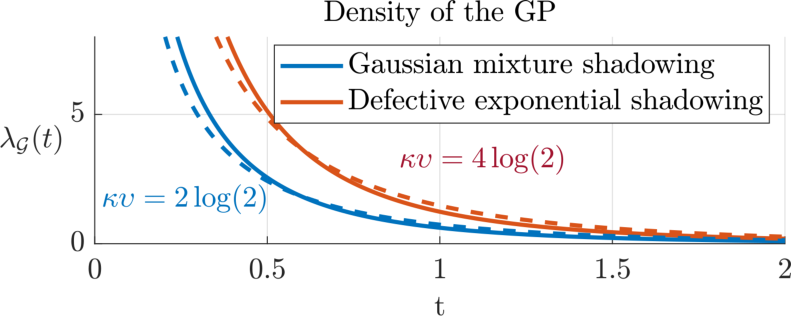
\includegraphics[width=\linewidth]{plotdensities.pdf}
           \caption{The density function of the GP with the mixture log-normal and defective exponential power shadowing models $H_{\mathcal{MLN}}$ and $H_{\text{Exp}}$, respectively. The values $\kappa \upsilon \in \{1.8,2.6\}$ were used. } 
           \label{fig:plotdensities}
         \end{figure}



The total interference, or total received power, is defined as the sum of the GP at the typical location $\textit{o}$ 
\begin{equation}
  \label{eq:totpow}
  I \triangleq \sum_{x \in \Phi} H_x G(\|x\|) = \sum_{x \in \mathcal{G}} x.
\end{equation}


The mean and the variance of $I$ are respectively given by
\begin{align}
  \label{eq:totmean}
  &\mathbb{E}\left(I \right) = \int_{0}^{\infty} t\lambda_{\mathcal{G}}(t) dt = \tilde{\kappa} \int_{0}^{\infty}F_H(t) dt =\tilde{\kappa} \mathbb{E}(H),
\end{align}
and
\begin{align}
  \label{eq:totvar}
  &\text{Var}\left(I \right) = \int_{0}^{\infty} t^2\lambda_{\mathcal{G}}(t) dt= \tilde{\kappa} \int_0^{\infty}tF_H(t) dt  \nonumber \\
  &= \tilde{\kappa} \frac{\text{Var}(H) + \mathbb{E}(H)^2}{2} = \tilde{\kappa}  \mathbb{E}[H^2]/2.
\end{align}


%% The spatial path loss is of no interest in the definition of $I$ because we assume that the spatial path loss is a constant due to the narrow-beam antenna pattern decaying fast to $0$, $G(\cdot)$, which ensures that the relevant UEs are located near one another (see Section \ref{sec:numericalresultsandconnectiontoLEO}). Hence, given that the spatial path loss is identical for all transmitters, it does not influence the SIR. For the SINR, the noise variable can be scaled appropriately to account for the spatial path loss appropriately. 







%% \subsection{Slow-fading distribution}
%% While analytically tractable, the defective exponential distribution can capture the mean and the variance of a more complicated fading distribution with high variance, particularly the lognormal distribution, which is a well-established shadowing model in the LEO networks. The shadowing is defined by the mixed exponential RV
%% \begin{equation}
%%   \hat{H}_x \sim
%%   \begin{cases}
%%     0, \text{ if } U < 1-\rho,\\
%%     \text{Exp}(\mu), \text{ if } U \geq1- \rho,              \label{eq:tier2exponential}
%%   \end{cases}
%% \end{equation}
%% with $\mu>0$ and $0<\rho\leq1$, and $U \sim U(0,1)$ follows the uniform distribution.


%%where
%% \begin{align}
%%   &a=\frac{2 (p_{\text{LoS}}-1) e^{{\mu_{N\text{LoS}}}+\frac{{\sigma_{N\text{LoS}}}^2}{2}}-2 p_{\text{LoS}} e^{{\mu_{\text{LoS}}}+\frac{{\sigma_{\text{LoS}}}^2}{2}}}{(p_{\text{LoS}}-1) e^{2 \left({\mu_{N\text{LoS}}}+{\sigma_{N\text{LoS}}}^2\right)}-p_{\text{LoS}} e^{2 \left({\mu_{\text{LoS}}}+{\sigma_{\text{LoS}}}^2\right)}},\\
%%   &b=\frac{2 \left(({p_\text{LoS}}-1) e^{{\mu_{\text{N\text{LoS}}}}+\frac{{\sigma_{\text{N\text{LoS}}}}^2}{2}}-{p_\text{LoS}} e^{{\mu_{\text{LoS}}}+\frac{{\sigma_{\text{LoS}}}^2}{2}}\right)^2}{({p_\text{LoS}}-1) e^{2 \left({\mu_{\text{N\text{LoS}}}}+{\sigma_{\text{N\text{LoS}}}}^2\right)}-{p_\text{LoS}} e^{2 \left({\mu_{\text{LoS}}}+{\sigma_{\text{LoS}}}^2\right)}}.              
%% \end{align} 



\subsection{Laplace transform of the total received power}

With exponential shadowing ${H}_{\text{exp}}$, for Re$(s)>1$,

\begin{align}
  \label{eq:lapdef}
  &\mathcal{L}_{I}(s)\triangleq \mathbb{E}\left(e^{-sI}\right)= \exp\left\{-\int_0^{\infty}(1-e^{-sr}) \lambda_{\mathcal{G}}(r) dr \right\} \nonumber \\
  &=\exp\left\{-\tilde{\kappa}\int_0^{\infty}(1-e^{-sr}) F_{{H}_{\text{exp}}}(r) /r dr \right\} \nonumber \\
  &=\exp\left\{-\tilde{\kappa}\upsilon_{}\int_0^{\infty}(1-e^{-sr}) e^{-r} /r dr \right\} =(1+s)^{-\tilde{\kappa}\upsilon_{}},
\end{align}
which is the Laplace transform of the gamma distribution with the shape parameter $\tilde{\kappa}\upsilon_{}$. 



\subsection{STIR process its factorial moment measures}
 We denote the signal-to-interference-plus-noise ratio (SIR) process of the UEs as
\begin{align}
  \label{eq:SINR}
  \Psi &= \{\mathsf{Z}: \mathsf{Z} \in \Psi\} \triangleq \left\{ \frac{u}{I-u} : u \in \mathcal{G}\right\} \nonumber \\
  &=\left\{ \frac{H_x G(D_{h,\epsilon}\|x\|)}{I-H_x G(D_{h,\epsilon}\|x\|)} : x \in \Phi\right\},
\end{align}
where $I$ is defined in \eqref{eq:totpow}. Similarly, the signal-to-total-interference ratio (STIR) process is defined as
\begin{align}
  \label{eq:STINR}
  \Psi' &= \{\mathsf{Z}': \mathsf{Z}' \in \Psi'\} \triangleq \left\{ \frac{u}{I} : u \in \mathcal{G}\right\}.
\end{align}
We can always recover on process from another
\begin{equation}
  \Psi = \left\{ \frac{\mathsf{Z}'}{1- \mathsf{Z}'}: \mathsf{Z}' \in \Psi' \right\}, \hspace{0.3cm} \Psi' = \left\{ \frac{\mathsf{Z}}{1+ \mathsf{Z}}: \mathsf{Z} \in \Psi \right\}.
\end{equation}
Let $\theta$ denote the SIR threshold of successful transmission. The event $\Psi \ni\mathsf{Z}> \theta$ is equivalent to $\Psi' \ni \mathsf{Z}'> \theta'$  with $\theta' \triangleq \theta/(1+\theta)$ and $\theta \triangleq \theta'/(1-\theta')$.

 The factorial moment measure of the STIR process is defined by,
    \begin{align}
          &M'^{(n)}(t'_1,\dots,t'_n) \triangleq M'^{(n)}((t'_1,\infty],\dots,(t'_n,\infty]) \nonumber \\
              &\triangleq \mathbb{E} \left( \sum^{\text{distinct}}_{\left(\mathsf{Z}'_1, \dots, \mathsf{Z}'_n \right) \in (\Psi')^{\times n}} \prod_{i=1}^n \mathds{1}(\mathsf{Z}'_i >t'_i)\right),
    \end{align}
    and similarly for the SIR process.
 The (partial) density of the factorial moment measure of the STIR process is given by the successive partial differentiation of $M'^{(n)}$:
    \begin{align}
      \label{eq:differatemomentmeasure}
     &{\mu'}_n^{(n+i)}(z'_1,\dots,z'_n,\overbrace{z'_n,\dots,z'_n}^{\#i}) \nonumber \\&= (-1)^n \frac{\partial^n M'^{(n)}(t'_1\dots t_n',z'_n \dots z'_n) }{\partial t'_1 \dots \partial t'_n} |(t'_1=z_1'\dots t'_n=z'_n),
    \end{align}
    for $\sum_{i=1}^n z'_i + i z'_n\leq 1$ and $0$ otherwise.  If $i >0$, $\eqref{eq:differatemomentmeasure}$ is the \textit{partial density} of the $n$th factorial moment measure.

    The density of the $n$th factorial moment measure of the SIR process can be extracted from $\mu'^{(n)}$:
    \begin{align}
      \label{eq:densitySINR}
      &\mu^{(n)}(z_1,\dots,z_n)&\\
      &= \prod_{j=1}^n\frac{1}{(1+z_j)^2}\mu'^{(n)}\left(\frac{z_1}{1+z_1},\dots,\frac{z_n}{1+z_n}\right)
    \end{align}

    
  
\subsection{Order statistics of the STIR process}
We denote $\mathsf{Z}'_{(1)}>\mathsf{Z}'_{(2)} >\mathsf{Z}'_{(3)} \dots$ the order statistics of the STINR process $\Psi'$, such that $\mathsf{Z}'_{(1)}$ is the larges value in $\Psi'$. Note that through the monotonicity of the relations \eqref{eq:STINR}, the order statistics of the STIR process is equivalent to the order statistics of the SIR process.

The joint pdf $k$ strongest values of the STIR process $(\mathsf{Z}'_{(1)}, \dots, \mathsf{Z}'_{(n)})$ is given as a series expansion involving the partial densities
\begin{equation}
  \label{eq:jointprobability}
  f'_{(k)}(z'_1,\dots,z'_k)= \sum^{i_{\text{max}}}_{i=0}\frac{(-1)^i}{i!}{\mu'}_k^{(k+i)}(z'_1,\dots,z'_k),
\end{equation}
for $z'_1>z'_2>\dots>z'_k$ and $f'_{(k)}(z'_1,\dots,z'_k) =0 $ otherwise. The upper bound for the index $i_{\text{max}}<1/z'_k-k$ is the non-zero terms of the series expansion. 

The $k$-coverage probability that the first $k$ strongest signals reach the threshold $\theta$ is given by
\begin{align}
  \label{eq:kprobability}
  &\mathcal{P}^{(k)}(\theta) \triangleq  \int_{\theta'}^1\dots \int_{\theta'}^1 f'_{(k)}({z'_1},\dots,{z'_k})dz'_1 \dots d{z'_k}, 
\end{align}
with $\theta'=\theta/(1+\theta)$ and $i_{\text{max}}<1/\theta'-k$.


\label{sec:partialdensitySIR}


\begin{prop}
  The density of the n\textit{th} factorial moment measure of the STIR process at a LEO BS with a narrow Gaussian antenna beam is given by
  \begin{align}
    \label{eq:factorialmoment}
    \mu'^{(n)}(t_1',\dots,t'_n) = (\tilde{\kappa}\upsilon_{})^n\prod_{j=1}^n{t'}_{j}^{-1}\left(1- \sum_{j=1}^nt'_j \right)^{\tilde{\kappa}\upsilon_{}-1},       
  \end{align}
  whenever $t_1>\dots >t_n$ and $\sum_{i=1}^n t_i \leq 1$, and $0$ otherwise.
  \begin{proof}
    The total interference follows a gamma proces, hence the STIR process can be characterized by a Poisson-Dirichlet distribution PD$(0,\tilde{\kappa}\upsilon)$ that has the corresponding density.
  \end{proof}
\end{prop}

The partial densities can be derived from the density of the $n$th factorial moment measure by integrating $\mu^{(n+i)}$ w.r.t. the last $i$ auxiliary variables (cf. \eqref{eq:differatemomentmeasure}).

\begin{align}
  \label{eq:auxillary}
  &{\mu'}_n^{(n+i)}(z'_1,\dots,z'_n) \nonumber \\
  &= \int_{z'_n}^1 \dots \int_{z'_n}^1 {\mu'}^{(n+i)}(z'_1,\dots,z'_n,\zeta'_1,\dots,\zeta'_i) d\zeta'_1 \dots d\zeta'_i,
\end{align}
the support of the density being in the region $\sum_{i=1}^nz'_i+iz'_n \leq 1$. 




\subsection{SIR under interference cancellation
}
Let $(u_{(1)}, \dots, u_{(k)}) \subset \mathcal{G}$ represent an ordered set of points in the GP, where $u_{(1)}$ denotes the strongest signal at the LEO BS. The signals with indices in the set $ \mathcal{K} \ni n,$  are canceled from the total interference. We denote the SIR under the interference cancellation (IC) as
\begin{equation}
  \label{eq:IC-SINR}
  \text{SIR}_{n,\mathcal{K}} \triangleq \frac{u_{(n)}}{I-\sum_{j \in [k]} u_{(j)}}.
\end{equation}
Under IC, we have the following identity in terms of the STIR process
\begin{equation}
   \mathbb{P}(\text{SIR}_{n,[k]} > \theta) = \mathbb{P}\left(\mathsf{Z}'_{(n)}+\theta'\sum_{j\in [k] \setminus \{n\}}\mathsf{Z}'_{(j)} > \theta'\right).
\end{equation}



%% \begin{align}
%%   \label{eq:IC-SINRcond}
%%   \mathcal{P}_{\text{IC}}^{(n,k)}(\theta) &\triangleq \mathbb{P}\{\text{SINR}_{n,k} > \theta \} \nonumber \\
%%   &=\mathbb{P} \left\{ u_{(n)} >\theta\left(N+I-  \sum_{j=1}^ku_{(j)}\right)\right\} \nonumber\\
%%   &\overset{}{=}\mathbb{P} \left\{(1+\theta) \frac{u_{(n)}}{N+1}+ \theta \frac{\sum^{j\neq n}_{j\in\{1,\dots,k\}} u_{(j)}}{N+I}>\theta \right\} \nonumber \\
%%   &\overset{(a)}{=} \mathbb{P} \left\{ \mathsf{Z}'_{(n)}+\theta'\sum^{j\neq n}_{j\in\{1,\dots,k\}}\mathsf{Z}'_{(j)} +>\theta'\right\}.
%% \end{align}

We consider the SIR under successive signal cancellation (SIC-SIR). The SIC-SIR at the n\textit{th} strongest UE with at most $K+n$ canceled signals, we denote the r.v. as SIR-SIC$_{n,K}$. A necessary condition for a successfully transmission from the $n$\textit{th} UE to the LEO BS is that the preceding $n$ signals are successively decoded and removed from the interference. Formally, $\{\mathsf{Z}_m'+\tau'\sum_{j=1}^{m-1}\mathsf{Z}_j'>\tau'\}$ for all $m \in \{1 \dots n\}$. The signal detection threshold is denoted as $ \tau = \tau'/(1-\tau') \leq \theta$. When the first $n$ signals are successfully removed from the interference, the $n$\textit{th} UE is in coverage if SIR$_{n,[n]}>\theta$. If it is not, we adapt an opportunistic, or adaptive, SIR-SIC scheme. Namely, the BS continues the interference cancellation $\{\text{SIR}_{n,[n]} \dots \text{SIR}_{n,[k]}  \}_{n\leq k \leq K}$ until SIR$_{n,[k]}>\theta$, or the served UE enters an outage if $\text{SIR}_{n,[n]} <\tau$, or the maximum number of canceled signals, $K=k-n$, is reached. It is not possible boundlessly improve SIC-SIR$_{n,K}$ as $K \rightarrow \infty$ because, in practical applications, $\mathbb{P}(\text{SIR-SIC}_{n,K}>\theta)$ does not improve after some $K$.

\begin{prop}
  Consider the adaptive SIC with at most $n+K$ canceled signals. The coverage probability of the UE with n\textit{th} strongest signal is given by
  \begin{align}
    &\mathcal{P}^{(n,K)}_{\textup{AD-SIC}}(\theta,\tau) \triangleq \sum_{k=n}^{K}\Delta^{(n,k)}_{\textup{SIC}}(\theta,\tau),
  \end{align}
  where
  \begin{align}
    \label{eq:SICprob}
    & \Delta^{(n,k)}_{\textup{SIC}}(\theta,\tau) \triangleq \sum^{i_{\text{max}}}_{i=0}\frac{(-1)^i}{i!} \int_{0}^{1} \dots \int_{0}^{1}\prod_{m=1}^k  \nonumber \\
    &\hspace{0.5cm}\mathds{1}\left( z'_m+ \tau'\sum_{j=1}^{m-1} z'_j>\tau' \right)  \mathds{1}\left(z'_n+  \theta'\sum_{j\in [k] \setminus \{n\}} z'_j>\theta' \right) \nonumber \\
    &\times \left(\mathds{1}(k>n)\mathds{1}\left(z'_n+ \theta'\sum_{j \in [k-1] \setminus \{n\}} z'_j<\theta' \right) + \mathds{1}(k=n) \right) \nonumber\\
    & \times \mathds{1}(z'_1>\dots>z'_k){\mu'}_k^{(k+i)}(z'_1,\dots,z'_k) d z'_1 \dots d z'_k,
  \end{align}
  with the upper summation limit bounded by $i_{\text{max}} < 1/\tau'-1=1/\tau$.
  \begin{proof}
    The expression follows from the joint pdf of the order statistics \eqref{eq:jointprobability} by imposing the conditions \eqref{eq:IC-SINRcond} and \eqref{eq:SIC-SINRcond}. We have abbreviated the upper bound of $i_{\text{max}}$ to $1/\tau$ from the upper limit given in \eqref{eq:jointprobability}: $i_{\text{max}} < 1/z'_{k}-k‰$, and $i_{\text{max}} \rightarrow \infty$ as $z'_k \rightarrow 0$. Fortunately, the l.h.s. conditioning limits the support of the integrand for small $z'_k$. Namely, a necessary condition is $z'_{k}+\tau'\sum_{j=1}^{k-1}z'_{j}>\tau'$. By simple algebra, $\sum_{j=1}^{k-1}z_{j}> 1-z_{k}/\tau'$. Recall the condition on the non-zero terms of the density of $M'^{(k+i)}$:  $\sum_{j=1}^k z'_{j}+i z'_{k} =\sum_{j=1}^{k-1}z'_{j} +z'_{k}+i z'_{k}  \leq 1$. The condition certainly does \textit{not} hold if $1-z_{k}/\tau'+ z'_{k}+i z'_{k}>1$. We arrive at the inequality $z'_{k} \left(-1/\tau' + 1 +i \right)>0$. Divide both sides by $z'_{k}$, and the general upper bound of $i$ follows.
  \end{proof}
\end{prop}


Combining \eqref{eq:densitySINR}, \eqref{eq:jointprobability}, and \eqref{eq:factorialmoment}, we get a closed form for the SIR pdf of the strongest signal in the \textit{simple coverage region} $z\geq 1$; $f_{(1)}(z) =  {\tilde{\kappa}\upsilon_{}\left({z + 1} \right)^{-\tilde{\kappa}\upsilon_{}}}/{z}$. An upper bound for the second moment is given by
\begin{equation}
  \label{eq:SIR1}
\mathbb{E}(\text{SIR}^2_{1,\{1\}}) \geq \int_{1}^{\infty}f_{(1)}(z) z^2 = \frac{2^{1-\tilde{\kappa}v}(\tilde{\kappa}v)^2}{(\tilde{\kappa}\upsilon-1)(\tilde{\kappa}\upsilon-2)},
\end{equation}
which converges for $\tilde{\kappa}\upsilon > 2$. Similarly for the second moment, $\mathbb{E}(\text{SIR}_{1,\{1\}})  = {2^{1-\tilde{\kappa}v}\tilde{\kappa}v}/{(\tilde{\kappa}\upsilon-1)},\tilde{\kappa}\upsilon>1$ which, \textit{i.e.}, for less than $2\log(2)$ effective UEs inside a $-3$ dB footprint on average. Despite of high average SIR, the infinite variance for $\tilde{\kappa}\upsilon \leq 2$ is unacceptable if we desire a consistent link quality. However, SIR-SIC can achieve similar performance while decreasing the variance. Furthermore, using signal cancellation the typical LEO BS can have better connection to the other UEs, not only the strongest. Furthermore, following from the order $\mathsf{Z}'_1 > \mathsf{Z}'_2 >\dots $, if $\mathsf{Z}'_1$ has a finite variance, then all other STIR values have also. This holds also for the sums of the variables, and hence for the AD-SIC.

Upper




  
\begin{figure}[h]
  \centering
  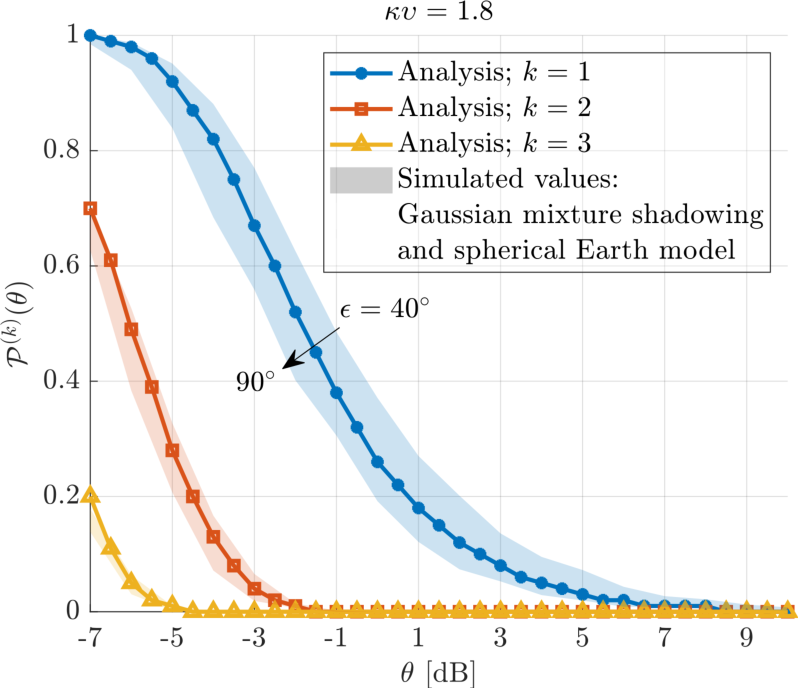
\includegraphics[width=\linewidth]{kprobabilities.pdf}
  \caption{The $k$-probabilities for $k \in \{1,2,3\}$ for $\kappa v=1.8$ (recall, $\kappa v$ corresponds to the average number of \textit{effective} UEs inside the SBS $3$ dB footprints). For the simulated values, the two-tier Gaussian mixture shadowing for $\kappa \upsilon_{} \in (1.8,2.6)$.
} 
  \label{fig:antennapats}
\end{figure}


In figures \ref{kprobabilities.pdf} we plot the probabilities for $\tilde{\kappa}\upsilon=2$ and  $\tilde{\kappa}\upsilon=7/2=3.5$.






%% \begin{verbatim}
%% \begin{table}
%% \begin{center}
%% \caption{Filter design equations  ...}
%% \label{tab1}
%%     \begin{tabular}{| c | c | c |c|}
%%       \hline
%%       & $\mathcal{P}^{(1)}(\cdot)$& $\mathcal{P}^{(2)}_{\text{IC}}(\cdot)$& $\mathcal{P}^{(2)}_{\text{SC}}(\cdot)$\\
%%       \hline
%%       $\mathbb{E}(\cdot)$&$1.4$ & $1.4$ &$1.4$\\ 
%%       \hline
%%       $\tilde{\kappa}$& $2/\upsilon_{} $ &$2.6/\upsilon_{}$& $3.4/\upsilon_{}$\\
%%       \hline
%%       Var$(\cdot)$& $\infty$ & $2.6$ &$2.3$\\
%%       \hline 
%%     \end{tabular}
%% \end{center}
%% \end{table}
%% \end{verbatim}


\appendices




\section{Scaling constant}


\label{app:constantD}
See Figure \ref{fig:triangle}. We have that $\zeta_{z}= \tan^{-1}(z/h)$. The derivative of $\varphi_x$  around $\textit{o}$ is given approximately by
\begin{align}
  &\frac{d}{d \| x\|}\varphi_{x} =\frac{d}{dz}\zeta_{z}  = \frac{d\tan^{-1}(z/h)}{dz} = \frac{h}{h^2 + z^2}   \nonumber\\
  %%              \end{align}
  %%            \begin{align}
  &\overset{(a)}{\approx} \frac{h}{h^2 -h^2 + \hat{d}^2_{h,\epsilon}}  \overset{(b)}{=}\frac{h}{ h^2/\sin^2(\epsilon)} = \frac{\sin^2(\epsilon)}{h} = D_{h,\epsilon},
  %%               & ,
\end{align}
where (a) follows from Pythagoras's theorem, and (b) is standard trigonometry.

\begin{figure}[h]
  \centering
  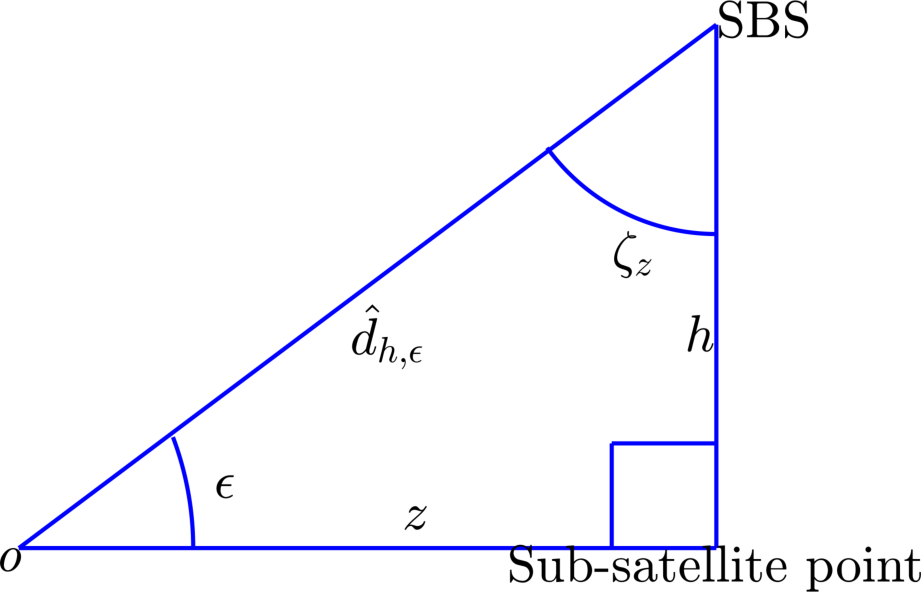
\includegraphics[width=0.7\linewidth]{triangle.pdf}
  \caption{Geometric interpretation of the variables in Appendix \ref{app:constantD} }
  \label{fig:triangle}
\end{figure}






\bibliographystyle{IEEEtran}
%\bibliography{IEEEabrv, bib}
\bibliography{IEEEabrv,source}


\end{document}
 
